\section{第6章\quad 实用微波传输线与波导}
\begin{frame}{第6章\quad 实用微波传输线与波导}
    \begin{itemize}
        \item 微波工程分析方法
              \begin{itemize}
                  \item 场论的方法
                  \item 网络的方法
              \end{itemize}
    \end{itemize}
    \begin{itemize}
        \item 传输线理论 $\Longrightarrow$ 波导
              \begin{itemize}
                  \item 当其他人或物靠近双导线时会产生较大影响。这说明,传输线与外界有能量交换,它带来的直接问题是能量损失和工作不稳定。就其原因是\textbf{开放(Open)}造成的特点
              \end{itemize}
    \end{itemize}
\end{frame}

\begin{frame}{第6章\quad 实用微波传输线与波导}
    \begin{itemize}
        \item 波导(Waveguide)构成
    \end{itemize}
    双导线两侧连续加对称$\lambda/4$支节,直到构成封闭(Closed)电路为止。如果其导线的宽度是$W$,则波导宽边
    \begin{align*}
        a=W+2\cdot \frac{\lambda}{4}=W+\frac{\lambda}{2} \\
        a\geqslant \lambda/2 或 \lambda\leqslant 2a
    \end{align*}
    这构成了波导传输的第一个约束条件 \\
    \centering
    \begin{figure}
        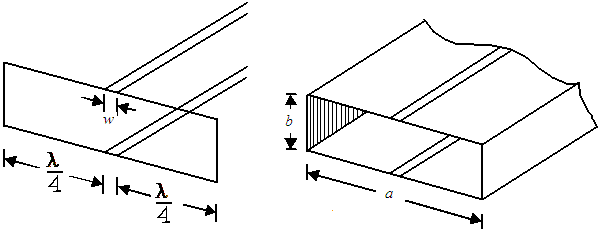
\includegraphics[width=6cm]{Cha6//fig6-0.png}
        \caption{从双导线到矩形波导}
    \end{figure}
\end{frame}

\subsection{预备知识}
\begin{frame}{预备知识}
    \begin{itemize}
        \item 交变电磁场基本关系式
    \end{itemize}
    \begin{align*}
        \begin{cases}
            \nabla\times\vec{E}=-\dfrac{\partial \vec{B}}{\partial t}\\
            \nabla\times\vec{H}=\dfrac{\partial \vec{D}}{\partial t}+\vec{J}\\
            \nabla\cdot\vec{D}=\rho\\
            \nabla\cdot\vec{B}=0
        \end{cases}
    \end{align*}
    \begin{align*}
        \vec{D}=\epsilon\vec{E},\vec{B}=\mu\vec{H},\vec{J}=\sigma\vec{E}
    \end{align*}
    无源区,时谐场
    \begin{align*}
        \begin{cases}
            \nabla\times\vec{E}=-\rm{j}\omega\mu\vec{H}\\
            \nabla\times\vec{H}=\rm{j}\omega\epsilon\vec{E}\\
            \nabla\cdot\vec{D}=0\\
            \nabla\cdot\vec{B}=0
        \end{cases}
    \end{align*}
\end{frame}

\begin{frame}{预备知识}
    \begin{itemize}
        \item 边界条件
    \end{itemize}
    \begin{columns}
        \begin{column}{0.5\linewidth}
            两种媒质界面的边界条件
            \begin{align*}
                \begin{cases}
                    \hat{n}\times(\vec{E_2}-\vec{E_1})=0\\
                    \hat{n}\times(\vec{H_2}-\vec{H_1})=\vec{J_s}\\
                    \hat{n}\cdot(\vec{D_2}-\vec{D_1})=\rho_s\\
                    \hat{n}\cdot(\vec{B_2}-\vec{B_1})=0
                \end{cases}
            \end{align*}
        \end{column}
        \begin{column}{0.5\linewidth}
            理想导体表面的边界条件
            \begin{align*}
                \begin{cases}
                    \hat{n}\times\vec{E_2}=0\\
                    \hat{n}\times\vec{H_2}=\vec{J_s}\\
                    \hat{n}\cdot\vec{D_2}=\rho_s\\
                    \hat{n}\cdot\vec{B_2}=0
                \end{cases}
            \end{align*}
        \end{column}
    \end{columns}
\end{frame}

\begin{frame}
    \begin{itemize}
        \item 交变电磁场的能量关系
    \end{itemize}
    对于一封闭曲面S,电磁场的能量关系满足复功率定理,即
    \begin{align*}
        -\oint_S\frac{1}{2}(\vec{E}\times\vec{H^*})\cdot\hat{n}\rm{d}S=P_L+\rm{j}2\omega(W_m-W_e)
    \end{align*}
\end{frame}

\begin{frame}{预备知识}
    \begin{itemize}
        \item 导波系统波形\\
              导波系统中的电磁波按纵向场分量的有无,分为以下三种波形(模)
              \begin{itemize}
                  \item 横磁波(TM波),又称电波(E波): $H_z=0,E_z\neq 0$
                  \item 横电波(TE波),又称磁波(H波): $E_z=0,H_z\neq 0$
                  \item 横电磁波(TEM波): $E_z=0,H_z=0$
              \end{itemize}
    \end{itemize}
\end{frame}

\begin{frame}{预备知识}
    \begin{itemize}
        \item 波导一般解的出发点和假定条件\\
              波导一般解的出发点是频域Maxwell方程组
              \begin{align}
                  \begin{cases}
                      \nabla\times\vec{H}=\rm{j}\omega\epsilon\vec{E} \\
                      \nabla\times\vec{E}=-\rm{j}\omega\mu\vec{H}     \\
                      \nabla\cdot\vec{E}=0                            \\
                      \nabla\cdot\vec{H}=0
                  \end{cases}
                  \label{eqn6-1}
              \end{align}
              波导假定条件
              \begin{columns}
                  \begin{column}{0.5\linewidth}
                      \begin{itemize}
                          \item 波导均匀条件:假定横截面不随$z$而变化
                          \item 媒质均匀条件:波导内部$\epsilon,\mu$均匀,波导内壁$\sigma$无限大
                          \item 无源条件:波导内$\rho,\vec{J}\equiv 0$
                          \item 无限条件:波导在$z$方向无限长
                      \end{itemize}
                  \end{column}
                  \begin{column}{0.5\linewidth}
                      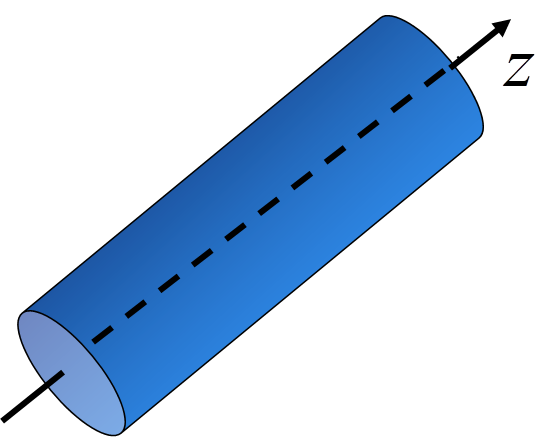
\includegraphics[width=5cm]{Cha6//fig6-1.png}
                  \end{column}
              \end{columns}
    \end{itemize}
\end{frame}

\subsection{矩形波导}

\begin{frame}{矩形波导}
    \begin{itemize}
        \item 矩形波导的一般解
    \end{itemize}
    (\ref{eqn6-1})第二式两边取旋度
    \begin{align*}
        \nabla\times\nabla\times\vec{E} & =\nabla(\nabla\cdot\vec{E})-\nabla^2\vec{E}=-\rm{j}\omega\mu\nabla\times\vec{H} \\
                                        & =\omega^2\mu\epsilon\vec{E}=k^2\vec{E}\\
                                        &k=\omega\sqrt{\mu\epsilon}=2\pi/\lambda
    \end{align*}
    得到波动方程
    \begin{align}
        \begin{cases}
            \nabla^2\vec{E}+k^2\vec{E}=0 \\
            \nabla^2\vec{H}+k^2\vec{H}=0 \\
        \end{cases}\label{eqn6-2}
    \end{align}
\end{frame}

\begin{frame}{矩形波导}
    \begin{itemize}
        \item 纵向场表示横向场
    \end{itemize}
    \centering
    \begin{figure}
        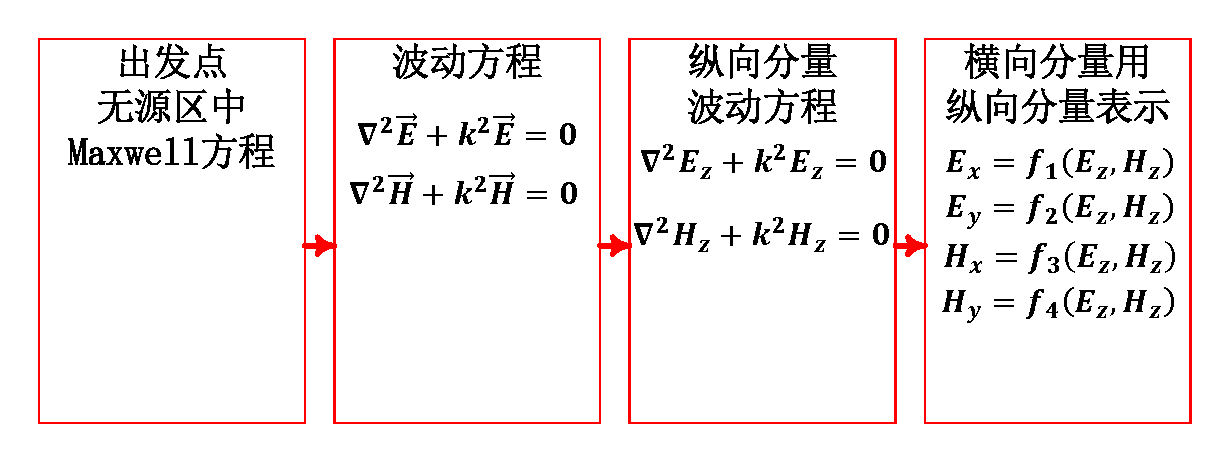
\includegraphics[width=10cm]{Cha6/fig6-2.pdf}
        \caption{纵向分量法流程图}   %\numberwithin{figure}{section}
    \end{figure} 
\end{frame}

\begin{frame}{矩形波导}
    纵向分量方程
    \begin{align}
        \begin{cases}
            \nabla^2E_z+k^2E_z=0\\
            \nabla^2H_z+k^2H_z=0
        \end{cases}
        \label{eqn6-3}
    \end{align}
    假定$E_z$或$H_z$可分离变量,即
    \begin{align}
        \begin{cases}
            E_z=E(x,y)Z(z)\\
            H_z=H(x,y)W(z)
        \end{cases}
        \label{eqn6-4}
    \end{align}
    且$Laplace$算子$\nabla^2$可分解为
    \begin{align}
        \nabla^2=\nabla_t^2+\frac{\partial^2}{\partial z^2}
        \label{eqn6-5}
    \end{align}
    将式(\ref{eqn6-4})、式(\ref{eqn6-5})代入式(\ref{eqn6-3})可知
\end{frame}

\begin{frame}{矩形波导}
    \begin{align}
        \frac{\nabla^2_t E(x,y)}{E(x,y)}+\frac{1}{Z(z)}\frac{\rm{d}^2 Z(z)}{\rm{d}z^2}+k^2=0
        \label{eqn6-6}
    \end{align}
    由于其独立性,上式各项均为常数
    \begin{align}
        \begin{cases}
            \dfrac{1}{Z(z)}\dfrac{\rm{d}Z(z)}{\rm{d}z^2}=\gamma^2\\
            \dfrac{\nabla_t^2E(x,y)}{E(x,y)}+k_c^2=0
        \end{cases}
        \label{eqn6-7}
    \end{align}
    其中
    \begin{align}
        k_c^2=k^2+\gamma^2
    \end{align}
    称为\textbf{截止波数}
\end{frame}

\begin{frame}{矩形波导}
    式(\ref{eqn6-7})中第一方程的解是
    \begin{align}
        Z(z)=C_1\rm{e}^{-\gamma z}+C_2\rm{e}^{\gamma z}
    \end{align}
    $$\downarrow$$
    \begin{align}
        \begin{cases}
            E_z=E(x,y)\rm{e}^{-\gamma z}\\
            H_z=H(x,y)\rm{e}^{-\gamma z}
        \end{cases}
    \end{align}
    $$\frac{\partial}{\partial z}\rightarrow -\gamma$$
\end{frame}

\begin{frame}{矩形波导}
    \begin{align*}
        \nabla\times\vec{H}=\rm{j}\omega\epsilon \vec{E} 
    \end{align*}
    \begin{align*}
        &\begin{vmatrix}
            \hat{x}                     & \hat{y}                     & \hat{z} \\
            \dfrac{\partial}{\partial x} & \dfrac{\partial}{\partial y} & -\gamma \\
            H_x                         & H_y                         & H_z     \\
        \end{vmatrix}
        =\rm{j}\omega\epsilon(\hat{x}E_x+\hat{y}E_y+\hat{z}E_z)
    \end{align*}
    \begin{align}
        \begin{cases}
            \dfrac{\partial H_z}{\partial y}+\gamma H_y=\rm{j}\omega\epsilon E_x\\
            -\gamma H_x-\dfrac{\partial H_z}{\partial x}=\rm{j}\omega\epsilon E_y\\
            \dfrac{\partial H_y}{\partial x}-\dfrac{\partial H_x}{\partial y}=\rm{j}\omega\epsilon E_z
        \end{cases}
    \end{align}
\end{frame}

\begin{frame}{矩形波导}
    \begin{align*}
        \nabla\times\vec{E}=-\rm{j}\omega\mu \vec{H} 
    \end{align*}
    \begin{align*}
        \begin{vmatrix}
            \hat{x}                     & \hat{y}                     & \hat{z} \\
            \dfrac{\partial}{\partial x} & \dfrac{\partial}{\partial y} & -\gamma \\
            E_x                         & E_y                         & E_z     \\
        \end{vmatrix}
        =-\rm{j}\omega\mu(\hat{x}H_x+\hat{y}H_y+\hat{z}H_z)
    \end{align*}
    \begin{align}
        \begin{cases}
            \dfrac{\partial E_z}{\partial y}+\gamma E_y=-\rm{j}\omega\mu H_x\\
            -\gamma E_x-\dfrac{\partial E_z}{\partial x}=-\rm{j}\omega\mu H_y\\
            \dfrac{\partial E_y}{\partial x}-\dfrac{\partial E_x}{\partial y}=-\rm{j}\omega\mu H_z
        \end{cases}
    \end{align}
\end{frame}

\begin{frame}{矩形波导}
    先整理$E_x,H_y$方程组,得
    \begin{align*}
        \begin{cases}
            \rm{j}\omega\epsilon E_x-\gamma H_y=\dfrac{\partial H_z}{\partial y}\\
            -\gamma E_x+\rm{j}\omega\mu H_y=\dfrac{\partial E_z}{\partial x}\\
        \end{cases}
    \end{align*}
    \begin{align*}
        D=
        \begin{vmatrix}
            \rm{j}\omega\epsilon & -\gamma \\
            -\gamma & \rm{j}\omega\mu\\
        \end{vmatrix}
        =-k^2-\gamma^2=-k_c^2
    \end{align*}
    \begin{align*}
        D_x=
        \begin{vmatrix}
            \dfrac{\partial H_z}{\partial y} & -\gamma \\
            \dfrac{\partial E_z}{\partial x} & \rm{j}\omega\mu\\
        \end{vmatrix}
        =\gamma\frac{\partial E_z}{\partial x}+\rm{j}\omega\mu\frac{\partial H_z}{\partial y}
    \end{align*}
    \begin{align*}
        D_y=
        \begin{vmatrix}
            \rm{j}\omega\epsilon & \dfrac{\partial H_z}{\partial y} \\
            -\gamma & \dfrac{\partial E_z}{\partial x}\\
        \end{vmatrix}
        =\rm{j}\omega\epsilon\frac{\partial E_z}{\partial x}+\gamma \frac{\partial H_z}{\partial y}
    \end{align*}
\end{frame}

\begin{frame}{矩形波导}
    \begin{align}
        \begin{cases}
            E_x=\dfrac{D_x}{D}=-\dfrac{1}{k_c^2}\left(\gamma\dfrac{\partial E_z}{\partial x}+\rm{j}\omega\mu\dfrac{\partial H_z}{\partial y}\right)\\
            H_y=\dfrac{D_y}{D}=-\dfrac{1}{k_c^2}\left(\rm{j}\omega\epsilon\dfrac{\partial E_z}{\partial x}+\gamma\dfrac{\partial H_z}{\partial y}\right)
        \end{cases}
        \label{eqn6-13}
    \end{align}
\end{frame}

\begin{frame}{矩形波导}
    再整理$E_y,H_x$方程组,得
    \begin{align*}
        \begin{cases}
            \rm{j}\omega\epsilon E_y+\gamma H_x=-\dfrac{\partial H_z}{\partial x}\\
            \gamma E_y+\rm{j}\omega\mu H_x=-\dfrac{\partial E_z}{\partial y}
        \end{cases}
    \end{align*}
    \begin{align*}
        D=
        \begin{vmatrix}
            \rm{j}\omega\epsilon & \gamma \\
            \gamma & \rm{j}\omega\mu\\
        \end{vmatrix}
        =-k^2-\gamma^2=-k_c^2
    \end{align*}
    \begin{align*}
        D_y=
        \begin{vmatrix}
            -\dfrac{\partial H_z}{\partial x} & \gamma \\
            -\dfrac{\partial E_z}{\partial y} & \rm{j}\omega\mu\\
        \end{vmatrix}
        =\gamma\frac{\partial E_z}{\partial y}-\rm{j}\omega\mu\frac{\partial H_z}{\partial x}
    \end{align*}
    \begin{align*}
        D_x=
        \begin{vmatrix}
            \rm{j}\omega\epsilon & -\dfrac{\partial H_z}{\partial x} \\
            \gamma & -\dfrac{\partial E_z}{\partial y}\\
        \end{vmatrix}
        =-\rm{j}\omega\epsilon\frac{\partial E_z}{\partial y}+\gamma \frac{\partial H_z}{\partial x}
    \end{align*}
\end{frame}

\begin{frame}{矩形波导}
    \begin{align}
        \begin{cases}
            E_y=\dfrac{D_y}{D}=\dfrac{1}{k_c^2}\left(-\gamma\dfrac{\partial E_z}{\partial y}+\rm{j}\omega\mu\dfrac{\partial H_z}{\partial x}\right)\\
            H_x=\dfrac{D_x}{D}=\dfrac{1}{k_c^2}\left(\rm{j}\omega\epsilon\dfrac{\partial E_z}{\partial y}-\gamma\dfrac{\partial H_z}{\partial x}\right)
        \end{cases}
        \label{eqn6-14}
    \end{align}
    把(\ref{eqn6-13})和(\ref{eqn6-14})进一步归纳成矩阵形式,得
    \begin{align}
        \begin{bmatrix}
            E_x\\
            E_y\\
            H_x\\
            H_y\\
        \end{bmatrix}
        =\frac{1}{k_c^2}
        \begin{bmatrix}
            -\gamma & 0 & 0 & -\rm{j}\omega\mu\\
            0 & -\gamma & \rm{j}\omega\mu & 0 \\
            0 & \rm{j}\omega\epsilon & -\gamma & 0\\
            -\rm{j}\omega\epsilon & 0 & 0 & -\gamma\\
        \end{bmatrix}
        \begin{bmatrix}
            \dfrac{\partial E_z}{\partial x}\\
            \dfrac{\partial E_z}{\partial y}\\
            \dfrac{\partial H_z}{\partial x}\\
            \dfrac{\partial H_z}{\partial y}\\
        \end{bmatrix}
    \end{align}
    $$\epsilon=\epsilon_0\epsilon_r(1-\rm{j}\tan\delta)$$
    $$\text{损耗角正切:} \tan\delta=\sigma/\omega\epsilon_0\epsilon_r$$
\end{frame}

\begin{frame}{矩形波导}
    \begin{itemize}
        \item 矩形波导的横向解
    \end{itemize}
    在矩形波导中存在TE和TM两类模,这里以TE模为例进行讨论,即$E_z=0$,对于纵向分量只需讨论$H_z$
\end{frame}

\subsection{圆波导}
\begin{frame}{圆波导}

\end{frame}

\subsection{同轴线}
\begin{frame}{同轴线}

\end{frame}

\subsection{平面传输线}
\begin{frame}{平面传输线}
    上世纪六十年代以来,在微波工程和微波技术上,出现了一次不小的革命,即所谓MIC(Microwave Integrated Circuit)微波集成电路——HMIC、MMIC。其特色是体积小、功能多、频带宽,但承受功率小。因此被广泛应用于接收机和小功率元件中,并都传输TEM波。\\
    作为这一革命的“过渡人物”是带状线(Stripline)。它可以看作是同轴线的变形。
\end{frame}






